\chapter{Charles's Law}

\section{Aim}
To determine the relationship between volume and temperature of a gas

\section{Background Information}
Gasses are all around us and are used in industrial and commercial objects such as tires, balls, balloons etc. Each one of these objects requires a certain volume of air to operate properly. Also, volume and temperature are fundamental variables used in daily life and therefore it is important to know if there is some relationship between the two in a gas. However, there might also be a relationship between the volume and pressure so careful consideration must be made to keep pressure constant during the experiment. If pressure is held constant what type of relationship is there between volume and temperature of a gas?

\section{Materials}
Bunsen burner, capillary tube sealed at one end, wire gauze, tripod stand, ruler, 2 rubber bands, thermometer, stirrer, sulfuric acid, water, large beaker. 

\section{Procedure}
\begin{enumerate}
\item Place a drop of sulfuric acid inside the capillary tube.
\item Tap the bottom of the tube until the acid is about $^2/_3$ the way down the tube.
\item Attach the tube to a ruler using two rubber bands.
\item Fill the beaker with water until it is about $^3/_4$ full.
\item Insert the ruler with the tube attached to it into the water so that nearly the whole tube is submerged. 
\item Put a thermometer and stirrer into the water of the beaker. Record the initial temperature $\theta_1$ of the water and the initial length $L_1$ of the air column which is below the sulfuric acid. 
\item Place a tripod stand over a Bunsen burner and then light the burner. 
\item Place wire gauze on top of the tripod stand. Then place the beaker, which has all of the other contents still in it, over the wire gauze in order to heat the water inside.
\item While stirring gently, record the length of the air column, $L_2$, after the water has heated $5^\circ$. 
\item Continue recording the length of the air column ($L_3$, $L_4$\ldots $L_6$) after each interval of $5^\circ$ increase of temperature. You should have a total of 6 readings when you finish the experiment.
\end{enumerate}

\begin{figure}[h!]
\centering
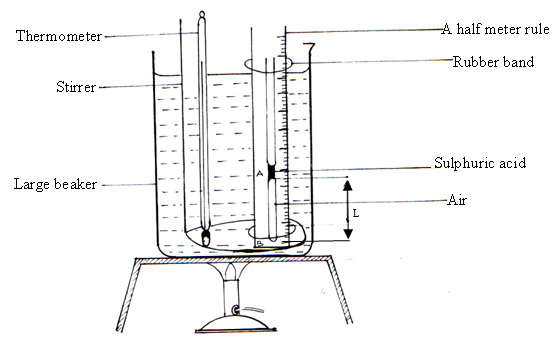
\includegraphics[width=12cm]{./img/charles-law-1.png}
\caption{Charles's Law practical setup}
\label{fig:charles-law-1}
\end{figure}

\section{Safety Measure}
Take care when using the Bunsen burner during the experiment.  

\section{Analysis and Interpretation}
\begin{enumerate}
\item Plot a graph of $L$ against $\theta$. What is the nature of the graph?
\item What is the approximate pressure of the air column during the experiment?
\end{enumerate}

\section{Conclusion}
What is the relationship between the volume and temperature of a gas when the pressure is held constant?

\section{Questions for Discussion}
\begin{enumerate}
\item What might happen to your results if you did not stir the water during the heating process?
\item Explain the purpose of the sulfuric acid drop in the capillary tube. Could something else have been used?
\item Does the mass of the air column remain constant? What about the density?
\end{enumerate}

\section{Reflection and Self Assessment}
\begin{enumerate}
\item Is there anything you do not understand about this experiment? If there is, what is it and in what ways can you increase your understanding?
\item What were the most and least interesting parts of the experiment to you? Explain.
\item Why are the results of this experiment necessary for the construction of tires?
\end{enumerate}